\documentclass[11pt]{article}  

\usepackage[utf8]{inputenc}
\usepackage{amsmath}
\usepackage[round]{natbib}
\usepackage{graphicx}
\usepackage{subcaption}
\usepackage{amssymb}
\usepackage[english]{babel}
\usepackage{array}
\usepackage{bbm}
\usepackage{mathpazo}
\usepackage{setspace}
\usepackage{booktabs}
\usepackage{algpseudocode}
\usepackage{libertine}
\usepackage{hyperref}
\usepackage{etoolbox}
\usepackage[table]{xcolor}
\usepackage{rotating}
\usepackage{grffile}
\usepackage{atbegshi}
\usepackage{longtable}
\usepackage{bbold}
\usepackage{caption}
\usepackage{titling}
\usepackage{url}
\usepackage{pgfgantt}

\usepackage[flushleft]{threeparttable}

\newcommand{\subtitle}[1]{%
  \posttitle{%
    \par\end{center}
    \begin{center}\large#1\end{center}
    \vskip0.5em}%
    }
\usepackage{graphicx}
\usepackage{subcaption}

\hypersetup{
    colorlinks=true,
    linkcolor=black,
    citecolor=blue!80!black,
    urlcolor=blue!80!black
}
     
\captionsetup[table]{name = Table}                        
\usepackage[margin=1in]{geometry}       
\geometry{a4paper, tmargin=2.5cm, bmargin=2.5cm, lmargin=2.5cm, rmargin=2.5cm}                   
\linespread{1.5}                                         

\usepackage{fancyhdr}
\usepackage{lipsum}

%%%%%%%%%%%%%%%%%%%%%%%%%%%%%%%%%%%%%%%%%%%%%%%%%%%%%%%%%%%%%%%%%%%


\begin{document}

\begin{titlepage}
   \begin{center}
       \vspace{1cm}

       \Large
       \textbf{ERASMUS UNIVERSITY ROTTERDAM}\\
       Erasmus School of Economics
            
       \vspace{0.5cm}
       \normalsize \textbf{Master Thesis} \\
       \textbf{Econometrics and Management Science}

       \vspace{1cm}
       \rule{\linewidth}{2pt}
       \Large 
       \textbf{Company Name Processing Fluency and Stock Characteristics:\\ A Deep Learning Approach}
       \rule{\linewidth}{2pt}
        
       \vspace{0.5cm}
       
    \end{center}
\\  
\begin{center}
Kevin Zhang \\
\small(538562)\\
\end{center}
\\
\begin{center}
Supervisor: dr. Flavius Frasincar\\        
Second assessor: dr. Wendun Wang\\
\end{center}
      
    \begin{center}
        \vspace{0.25cm}
        
                Date final version: \today

        \vspace{0.25cm} 

        \small 
        The views stated in this thesis are those of the 
        authors and not necessarily those of the 
        supervisor, second assessor, Erasmus School of 
        Economics, or Erasmus University Rotterdam.
            
   \vspace{0.5cm}
   
    \large 
    \textbf{Abstract}
   
   \end{center}
   The Latin phrase \textit{``nomen est omen"} says that someone's name can indicate their fate. In this paper, we have investigated that for company names. We have done this by training a deep neural network that predicts the processing fluency of words and names based on their features. For that, we use word frequency as proxy for its fluency. The trained model is then used to predict both fluency scores for a labelled test set and for names of firms that are listed on the New York Stock Exchange. Panel regressions are used to evaluate the effects of the firm name fluency predictions on stock valuation, liquidity, and performance. The out-of-sample performance of predicting the test observations is promising, as the model is able to beat its benchmarks.
   In the panel regressions, we find that the company name fluency scores only have significant effects in the case of valuation.


   
\noindent
\\
\small
\textbf{Keywords:} Processing Fluency, Behavioural Finance, Deep Learning, Econometrics, Quantitative Finance

\end{titlepage}

%%%%%%%%%%%%%%%%%%%%%%%%%%%%%%%%%%%%%%%%%%%%%%%%%%%%%%%%%%%%%%%%%%%


\newpage
\tableofcontents

\newpage
\listoffigures

\newpage
\listoftables


%%%%%%%%%%%%%%%%%%%%%%%%%%%%%%%%%%%%%%%%%%%%%%%%%%%%%%%%%%%%%%%%%%%





\newpage
\section{Introduction}
In traditional finance, one may notice the term \textit{homo economicus}. It translates to: economic human. The assumption here is that humans are rational, so that they make optimal choices. This concept is first introduced by \cite{mill1874essays} and its impact is substantial, as many studies have it as one of their core assumptions. For example, prestigious findings like the Markowitz model \citep{markowitz} or the Efficient Market Hypothesis \citep{fama1970efficient}, incorporate the assumption of rationality. However, by assuming perfect rationality, one leaves no room for possible behavioural biases. 

So, although the studies that rely on rationality have yielded many valuable insights, their ability in explaining market anomalies is still limited in some cases \citep{subrahmanyam2008behavioural}. The latter is partly the reason for the revival of behavioural finance \citep{kapoor2017behavioural}. Behavioural finance explains market anomalies with cognitive biases. Numerous studies have already done this. Among these studies, there is for instance the notable study by \cite{saunders1993stock} in which a relation between the weather in New York and the returns of equities listed on Wall Street is found. It states that equities are better performing during sunny days. The latter is likely due to the fact that weather indirectly influences the market by influencing the mood of its participants \citep{cunningham1979weather}. Another example is the study of \cite{shefrin1985disposition} in which they introduce the \textit{disposition effect}. This effect tells us that investors tend to sell well-performing stocks too soon and keep the ones that are doing poorly too long. An explanation can be found in \textit{prospect theory} \citep{kai1979prospect}. The main idea behind this theory is that people in general are more sensitive to losses than to gains. This explains why people are willing to take more risks when avoiding losses than when seeking gains.

We examine  another possible bias. We focus on the effect of a company's name on stock valuation, liquidity, and performance. The general idea of examining names in behavioural finance has been done by others before. For example, \cite{itzkowitz2017name} have done a study in which they show that private investors are more prone to behavioural biases like alphabetical ordering, company name fluency, and memorability than institutional investors.
\cite{kumar2015s} have found that U.S. mutual funds that are managed by managers with foreign-sounding names receive lower annual fund flows, even when the funds' performances are similar to the ones controlled by non-foreign-sounding managers. \cite{el2021s} have found that it is beneficial for mutual funds to make their name sound more sustainable. Funds that change their names receive higher fund flows in the periods thereafter, even after correction for performance. \cite{cooper2001rose} have investigated the effect of name changes during the dot-com bubble. They find that firms that adopt an Internet-related name change receive higher market appreciation.

Names are thus important and, for most of the time, it is the first thing a potential investor has to process when searching for investment opportunities. One can argue that first impressions could come with cognitive biases (e.g., \cite{hirshleifer2021first}). In addition, it is also quite intuitive for (retail) investors to be attracted to companies with better-sounding names.
So, we focus on this concept by looking at \textit{processing fluency}, which refers to the ease with which people can process and understand stimuli.
We hypothesise that company name fluency may have significant effects on stock characteristics.
To test our hypothesis, we shall answer the following question:
\vspace{0.25cm}
\begin{center}  
    \textit{Does a company's name fluency have significant effects on the company's stock characteristics?}
\end{center}
\vspace{0.25cm}

The motivation and features of the names in our approach come primarily from behavioural finance. We apply a deep learning model, due to its good performance in other studies, to link these features with a word's processing fluency. Once we have predictions of the processing fluency of a firm's name, we examine its effects with panel regressions.
The characteristics we focus on are valuation, liquidity, and performance of companies that are listed on the New York Stock Exchange. 
It turns out that, we do find significant effects of the predicted company name fluency scores in the case of valuation. For the other two characteristics, it is the control variables that are important.

These findings may be useful for both investors and academics. For instance, investors recognise the importance of data-driven insights \citep{yin2015big}, as these can be used to make better decisions.
This interest is also reflected in the vast increase in the number of academic publications published annually about (big) data applications in the field of finance. In the past ten years, we see that the number of English publications that deal with the application of data science in finance has increased from practically no interest to around 300 publications per year \citep{nobanee2021bibliometric}. We notice, however, that the studies that focus on company names make little to no use of machine learning. That is why
we contribute to the literature by using a deep learning model, which is trained on a frequency list, which in turn serves as a proxy for processing fluency.

The structure of this paper is as follows. First, we discuss related work in Section 2. Then, we present the data in Section 3. The proposed methods are explained in Section 4 and the results are reported in Section 5. Section 6 concludes the paper.

















\newpage
\section{Related Work}
First, we examine literature in the field of behavioural finance. That forms the foundation for what features we are going to construct. After that, we link those features with processing fluency. For that part, we primarily focus on deep learning (i.e., a neural network). The latter is because deep learning has already shown good performances in other studies.

\subsection{Behavioural Finance}
As we investigate whether the processing fluency of a company's name effects its stock characteristics, we first have to define what exactly processing fluency is. However, a word's processing fluency is quite abstract and subjective in the first place, as it could also depend on someone's literacy. 
\cite{reber2004processing} have worked out this concept more broadly and defined it as \textit{``the ease of mental operations concerned with stimulus meaning and its relation to semantic knowledge structures"}. In their work, they identify a set of properties that influence the processing fluency of a general stimulus:
\vspace{0.25cm}
\begin{itemize}
    \setlength\itemsep{-0.5em}
    \item Amount of Information; 
    \item Symmetry;              
    \item Contrast and Clarity;  
    \item Repetition;            
    \item Prototypicality.       
\end{itemize}
\vspace{0.25cm}
The \textit{Amount of Information} refers to the degree of complexity. Generally, individuals tend to favour simpler stimuli over challenging ones. The \textit{Symmetry} factor refers to the balance in the proportions of the stimuli. There are overlaps between complexity and symmetry. \cite{garner2014processing} has found that people prefer symmetrical figures over non-symmetrical ones. Symmetrical figures contain less information and are thus easier to process. \textit{Contrast and Clarity} are about how much the stimulus is distinct from its surroundings. \cite{reber1998effects} have found that people rate figures as prettier when they have higher figure-ground contrast. \textit{Repetition} is about the frequency of exposure. According to the \textit{mere-exposure effect} \citep{zajonc1968attitudinal}, more exposure results in more favourable evaluations. The final factor is \textit{Prototypicality}, which means that people tend to prefer more average or prototype-like stimuli over deviating ones. For example, \cite{langlois1990attractive} have found that composite faces are rated as more attractive than the faces that create those composites.

We choose to take the \textit{Repetition} factor as a proxy for word processing fluency. This factor is one of the least abstract ones, and it allows us to use word frequency as the proxy for its fluency. To give an intuition of this proxy, we consider the word \textit{`bike'}. Its semantics is for most of us directly clear, since it is one of the most important and used words in the English language\footnote{\url{https://www.oxfordlearnersdictionaries.com/wordlists/oxford3000-5000}}. Besides \textit{`bike'}, we could also use the less frequent form \textit{`bicycle'}, which can be somewhat harder to process for the inexperienced reader. Last, another synonym is \textit{`velocipede'}, which is even less used and harder to process. With the latter, one could also for instance erroneously associate a dinosaur (\textit{`velociraptor'}) or an insect (\textit{`centipede'}).

Other forms of labelled data have also been used before. This includes a series of studies done by \cite{alter2006predicting} in which they have investigated the relationship between firm name fluency and stock performance during the first year after its Initial Public Offering (IPO). In the first study, a group of undergraduates is asked to give their expectations about the future performance of some fictional stocks. The authors find that the participants expect more fluently named fictional stocks to outperform their non-fluent peers.
In a second study, the researchers confirm this result with real stock market data and find that a portfolio formed with the most fluent company names outperforms the one formed with the least fluent ones, even after controlling for other factors. 
In their third study, they also controlled for the meaning of firm names by using tickers only.
The results in their third study were similar to those found in their second one. \cite{jacobs2016alphabetic} used the alphabetical ordering of the company names as labels. They motivate their method with the \textit{primacy effect} \citep{carney2012first}. This effect states that people prefer things that appear earlier in a series. They find that U.S. firms that are alphabetically ranked higher, have higher trading activity and liquidity. They also evaluated the Japanese stock market as part of their robustness checks. There they  find a similar effect, which was not based on names, but based on Corporate Numbers instead. The latter is because stocks in Japan are sorted by identification number.

There is also the possibility of using unlabelled data. \cite{green2013company} have done this in their research. They calculated a fluency score based on the name itself. The score is a sum of three aspects: a length score, the \textit{Englishness score} \citep{travers1978pronounceability}, and a grammar check score. After controlling for other variables, they find that their fluency score significantly explains firm stock characteristics like valuation and liquidity. \cite{van2018company} followed the same summing approach and concludes that stocks with more fluent names generate higher abnormal returns, but they also mention that this effect is mostly concentrated among small firms and firms that are more sensitive to investor sentiment. 

Reviewing the literature, we conclude that our contribution is the fact that we introduce a novel proxy for word fluency, namely its frequency in a corpus. In addition, we also use machine learning to determine the fluency of words. The prior mentioned literature only work with surveys or heuristics.


\newpage
\subsection{Deep Learning for Processing Fluency}
So, we assume that frequency can be used as a proxy for processing fluency. Processing fluency in turn has a positive relationship with mental approval. This means, by transitivity, that words to which we are more exposed should generally be more positively mentally evaluated. \cite{reber1998effects} summarised this phenomenon as  \textit{``According to a two-step account of the mere-exposure effect, repeated exposure leads to the subjective feeling of perceptual fluency, which in turn influences liking"}. This mere-exposure effect is introduced by \cite{zajonc1968attitudinal}. In his study, he has found a positive correlation between the frequency of a stimulus and its evaluation. This effect is found in, among others, (fictional) words, symbols, and names. In our setting, this boils down to the fact that people process firm names more fluently when they are more exposed to (parts of) the name. \cite{green2013company} also have noticed this phenomenon in their study on firm name fluency. In an example they give, they mention that people could instinctively feel more comfortable investing in a fluently named company like \textit{Forest Laboratories} than investing in a non-fluent peer like \textit{Allergan Ligand Retinoid Therapeutics}.

Therefore, processing fluency has some commonalities with sentiments in sentiment analysis. Sentiment analysis is the computational study of human opinions, sentiments, and emotions, among other subjects \citep{liu2020sentiment}. In sentiment analysis, words and names may have polarity. Polarity refers to the connotation of a word or piece of text. For example, the connotation of the word \textit{`bad'} is considered to be negative, while the connotations of the words \textit{`chair'} and \textit{`benign'} are neutral and positive, respectively. However, in our case, we do not use the connotations of words derived from the semantics meant by the \textbf{messenger}. We focus on the ease with which a word can be processed by its \textbf{reader}. To be more specific, we concentrate on how the reader experiences a word after reading it, regardless of its meaning. For instance, in our setting, the words \textit{`bad'} and \textit{`benign'} are considered to be pleasant (easy) and unpleasant (hard) to process, respectively. The latter is because people are far more familiar with the former than with the latter\footnote{\url{https://www.oxfordlearnersdictionaries.com/wordlists/oxford3000-5000}}. This effect of fluency and easiness also appears in names, as  \cite{laham2012name} have found that easy-to-process names (and the persons who carry them) are judged more positively than persons with more difficult names.

Hence, we train a deep learning model that predicts this word fluency with the features of a given word. The reason we choose this approach is that the structure of a deep learning model allows us to learn complex and non-linear relationships in data by using multiple abstraction layers. Deep learning has already demonstrated its effectiveness in numerous scientific fields and applications, such as image classification, molecular biology, and natural language processing \citep{lecun2015deep}. The choice to use deep learning in our mental processing fluency setting may seem ad hoc. Yet, \cite{marblestone2016toward} argue that deep learning models are much more intertwined with neuroscience than we think. They state that brains do, just like deep learning models, optimise cost functions. A prominent example is \textit{Hebbian plasticity}
\citep{hebb2005organization}. It states that the connections between brain neurons are strengthened when they are used more frequently.
Brains also have cost functions that differ across places in the brain and over time. One of the examples \cite{marblestone2016toward} give is that we learn through social feedback and imitation that update our cost functions. 
Last, optimisation of those functions occurs in specialised brain tissue. Like specialised deep learning models, the brain has parts that are specialised for specific tasks.

\cite{abdul2017emonet} have applied specialised deep learning models to detect emotions in Twitter data. They use \textit{distant supervision} to acquire a proxy for the ground truth. Their study reveals that good to superior accuracy can be achieved with their approach compared to other related studies. 
\cite{salazar2020} used the pseudo log-likelihood scores derived from BERT masked language models and interpret these as a fluency proxy for sentences. An application of these scores in their study is to choose the most acceptable sentences in the minimal pairs datasets of Benchmark of Linguistic
Minimal Pairs (BLiMP). It turns out that their approach is able to achieve competitive performances compared to GPT-2 and human ratings. \cite{hu2021s} have trained character-based machine learning models (including deep neural networks) to predict gender based on the first names of Internet users. They conclude that their models achieve higher accuracy than baseline models that work with online user activity or name embedding. 

Our contribution to the stated literature is that we apply a machine learning approach for evaluating firm names in the field of behavioural finance. We do this by training a neural network that predicts the fluency of words and names.







\newpage
\section{Data}
In this study, we use 4 datasets. First, we have an extensive list of English words, which we call the \textit{lexicon}. Then, we have a labelled \textit{frequency list} of English words, which we use to train, validate, and test the deep learning model. Then, we let the trained deep learning model predict fluency scores of names in a \textit{list of company names}. At last, we evaluate those fluency predictions in panel regressions. The control variables in those regressions are from \textit{Compustat}. 


\subsection{Lexicon} \label{Lexicon}
The lexicon is a list of many English words. It serves as a source from which we can obtain statistics about the English language. With these statistics, we can create the first feature (i.e., \textit{Englishness score}) of the words and names in the frequency and company name list.

The lexicon we use comes from the \textit{words} module of the Natural Language Toolkit (NLTK) library\footnote{\url{https://www.nltk.org/}}. It is a list with about 236,000  English words. These words originate from a standard file found in Unix operating systems\footnote{\url{https://en.wikipedia.org/wiki/Words_(Unix)}}. To work with all these words in a standardised way, we first convert the capitalisation of each word to lowercase. After that, we lemmatise each word and keep only the unique lemmas. This de-biases the list from words that are similar due to their inflections (e.g., plural forms).
Last, we remove special characters and single letters. In total, we were left with 233,414 words after completing this process.



\subsection{Frequency List} \label{Training set}
The dataset with which we train the machine learning model is a frequency list. A frequency list is a list of words ranked by how frequently they occur in a corpus. The label of each word is its frequency, which in our case serves as a proxy for the word's processing fluency. We use this label as the target variable.  We aim to train a machine learning model that predicts this target variable as well as possible given the features of a word. The frequency list we use comes from the Centre for Translation Studies at the University of Leeds. The words in this list come from their Internet corpus\footnote{\url{http://corpus.leeds.ac.uk/list.html}}. In total, the original list contains 20,000 English words. In this dataset, we only remove the words that contain special characters or single letters. After this, we are left with 19,030 words. 





\subsection{Company Names}
Once the network is trained, we can use it to mimic the mental processing of words. The network takes as input the features of a word and returns an estimated fluency (frequency) as output.
We apply the trained model to assign fluency scores to names in a list of company names. This list contains names of companies that are listed on the New York Stock Exchange (NYSE) and it is obtained from the NASDAQ screener\footnote{\url{https://www.nasdaq.com/market-activity/stocks/screener}}. We decide to keep only the companies that exist for more than 10 years, as this ensures that we have enough observations to perform sufficiently reliable analyses. For each company in the list, we are only interested in the common stock listing. This means that we do not consider other assets such as mutual funds or double listings. We also omit the few companies that have numbers in their name.

After filtering based on the above-stated criteria, we preprocess the names of the remaining 1193 companies. Many of these end with legal terms (Corp., LLC, Inc., etc.). As these endings are rather standard and not decisive for distinguishing between names, we remove these endings. An exception to this rule is when a company is explicitly named with a legal term. Furthermore, we remove all special characters, punctuation, and single letters. Illustrative examples of name processing are given in Figure \ref{fig:preprocessing}.

\begin{figure}[h]
    \centering
    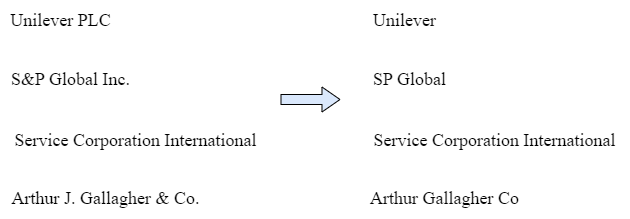
\includegraphics[scale=0.6]{figures/processing.png}
    \caption{Examples of preprocessing company names}
    \label{fig:preprocessing}
\end{figure}
\noindent


\subsection{Compustat}
As mentioned before, we use panel regression control variables from Compustat\footnote{\url{https://www.spglobal.com/marketintelligence/en/?product=compustat-research-insight}}. The panel data is collected on a monthly basis and range from January 2013 to December 2022. However, despite the extensiveness of Compustat, there are still companies which have missing or incomplete data. The regression ignores observations with missing values. So, to still perform fully balanced panel regressions, we only consider those companies for which we have complete data. This provides us with 202, 167, and 951 companies to work with in the liquidity, valuation, and performance regression, respectively.




\newpage
\section{Methods}
Our methods can be summarised in 3 main steps. In the first step, we train and evaluate the deep learning model. For that, we use standardised features of the words in the frequency list and we let the model use those features to fit the fluency (frequency) scores. In the second step, we use the trained model to predict the fluency scores of the firm names. In the last step, we regress the stock characteristics on the fluency predictions and control variables in order to estimate their effects. A visual illustration of the 3-step approach is given in Figure \ref{fig:overview}.

\vspace{0.5cm}
\begin{figure}[h]
    \centering
    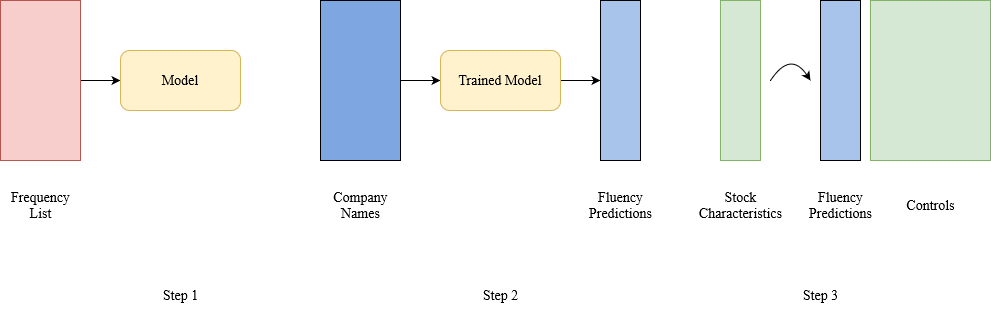
\includegraphics[scale=0.45]{figures/steps.png}
    \caption{Visual illustration of the 3-step approach}
    \label{fig:overview}
\end{figure}
\vspace{0.5cm}
\noindent
In the remainder of this section, we first discuss the inputs of the deep learning model. Then, we describe the deep learning model. Last, we describe the panel regressions.


\subsection{Features}
In the coming subsections, we discuss the inputs of the deep learning model. These inputs are features of the words and names for which we want to calculate the fluency score. For each feature, we explain its motivation and calculation.

\subsubsection{Englishness Score}
The \textit{Englishness score} \citep{travers1978pronounceability} measures how `English' a particular word is using conditional bi- and trigram probabilities. The measure evaluates a word as more English if it consists of bi- and trigrams that are more common in the English language. Following this concept, we use the Englishness score as the first feature. 

Let us denote an $n$-letter string as: $\#L_1L_2L_3,...,L_k,...,L_n\#$ in which $L_i$ stands for the $i$'th letter of the string. The symbol $\#$ indicates a space (spaces only occur at the beginning or end of a string). The Englishness score ($E$) is defined as the total conditional probability of the $n$-letter string:
\begin{equation}
    E = P(\#) \cdot P(L_1|\#) \cdot P(L_2|\#L_1) \cdot P(L_3|L_1L_2), ..., P(L_k|L_{k-2}L_{k-1}) , ..., P(\#|L_{n-1}L_{n})
\end{equation}
Each conditional probability can be estimated as
\begin{equation}
    P(L_k|L_{k-2}L_{k-1}) \approx \frac{F(L_{k-2}L_{k-1}L_k)}{F(L_{k-2}L_{k-1})}
\end{equation}
where $F$ denotes the number of occurrences of a bi- or trigram in the English language. We use the words in the \textit{lexicon} (see \hyperref[Lexicon]{Section 3.1}) to count the number of occurrences of each possible bi- or trigram.
If we substitute (2) into (1), we get an approximation of $E$
\begin{equation}
    E \approx \frac{F(\#)}{F(ALL)} \cdot \frac{F(\#L_1)}{F(\#)} \cdot \frac{F(\#L_1L_2)}{F(\#L_1)} \cdot \frac{F(L_1L_2L_3)}{F(L_1L_2)},..., \cdot \frac{F(L_{k-2}L_{k-1}L_k)}{F(L_{k-2}L_{k-1})}, ..., \frac{F(L_{n-1}L_n\#)}{F(L_{n-1}L_{n})}
\end{equation}
in which $F(ALL)$ is the count of all characters.
In the approximation, the terms $F(\#L_1)$ and $F(\#)$ are cancelled out. Furthermore, we ignore the $\frac{1}{F(ALL)}$ term since it is the same in every word, and therefore irrelevant for distinguishing between words. This simplifies (3) to:
\begin{equation}
    E' = F(\#L_1L_2) \cdot \frac{F(L_1L_2L_3)}{F(L_1L_2)},..., \cdot \frac{F(L_{k-2}L_{k-1}L_k)}{F(L_{k-2}L_{k-1})}, ..., \frac{F(L_{n-1}L_n\#)}{F(L_{n-1}L_{n})}
\end{equation}
We then take the natural log of expression (4) and multiply the outcome with -1. The result can be interpreted as a negative log-likelihood:
\begin{equation}\small
    E'' = - [ \text{log}(F(\#L_1L_2)) + \text{log}(\frac{F(L_1L_2L_3)}{F(L_1L_2)}) + ... + \text{log}(\frac{F(L_{k-2}L_{k-1}L_k)}{F(L_{k-2}L_{k-1})}) + ... + 
    \text{log}(\frac{F(L_{n-1}L_n\#)}{F(L_{n-1}L_{n})})]
\end{equation}

The Englishness score obtained in (5) is likely to be correlated with word length. \cite{travers1978pronounceability} controlled for this by dividing each word's $E''$ by the length of the word. \cite{green2013company} controlled for length by regressing the $E''$s on word length. They used the residuals of that regression as the Englishness score. In this paper, we follow the regression approach. If a name consists of multiple words, we calculate its Englishness score as the sum of the scores of the words that make up the name. The total name length is then calculated as the sum of the lengths of the words that make up the name.

We may also encounter words or names that contain bi- or trigrams that do not appear in the lexicon. This can cause the formula in (5) to become infeasible. To address this, we substitute a small conditional probability of 0.1\% if the bigram does not exist (if the bigram does not exist, its conditional trigrams do not exist either). If the prefix bigram does exist, but the conditional trigram does not, we use 1 divided by the number of bigrams as an ad hoc guess of the conditional probability. Some examples of the Englishness score of names are given in \hyperref[Appendix A]{Appendix A}.










\subsubsection{Word Length}

\cite{rennekamp2012processing} has found in an experiment that retail investors react stronger to news in company disclosures that are more legibly written. 
The study states that the readability effect may be related to processing fluency, as the amount of information that is presented to the participants remained the same in different versions of the disclosure.
More readable texts make readers process the content better and more easily, which in turn affects their sense of knowledge and perception of the company.
Like processing fluency, the definition of the readability of text is also rather subjective. \cite{kincaid1975derivation} have constructed formulas with which one can calculate the readability of documents. One feature in these formulas is the average amount of words per sentence. Since we do not work with documents, this feature translates to average word length. Some examples are given in Figure \ref{fig:wordlength}, where the numbers in brackets are the feature values.
\vspace{0.5cm}
\begin{figure}[h]
    \centering
    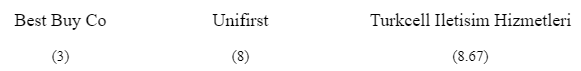
\includegraphics[scale=0.6]{figures/average_length.png}
    \caption{Examples of average word length}
    \label{fig:wordlength}
\end{figure}
%\vspace{0.5cm}

\subsubsection{Syllables}
The other feature in the formulas of \cite{kincaid1975derivation} is the average amount of syllables per word. Unlike the average amount of words per sentence, we can use this feature in our setting. By doing so, we notice that the average amount of syllables will sometimes be correlated with the average word length. Yet, We decide to use both since the focus of the two features is different. In addition, there are also cases in which this correlation seems not to hold. For example, the word \textit{`branch'} has 6 letters and 1 syllable, while the word \textit{`banana'} has 6 letters and 3 syllables. These cases might be valuable when training our model. Figure \ref{fig:averagesyllables} gives some examples of the average amount of syllables feature.

\vspace{0.5cm}
\begin{figure}[h]
    \centering
    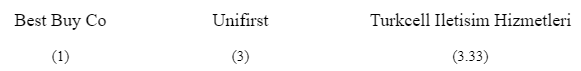
\includegraphics[scale=0.6]{figures/average_syllables.png}
    \caption{Examples of average syllables}
    \label{fig:averagesyllables}
\end{figure}
\vspace{0.5cm}










\subsubsection{Alphabetical Order}
\cite{jacobs2016alphabetic} have found that the alphabetical ordering of stocks significantly effects market characteristics. Stocks that appear alphabetically earlier  have higher turnover and liquidity. The latter is because investors only have limited awareness of all stocks available, and the alphabetical sorting of them may introduce an order bias in which a subset of firms is made more visible. To capture a potential ordering bias, we use one-hot encoding. The first variable is set to 1 if the first letter of a word is in the set \{\textit{a,b,c,d,e}\}, the second variable is set to 1 if this first letter is in \{\textit{f,...,u}\}. The last variable will be 1 if the first letter is in \{\textit{v,w,x,y,z}\}. In doing so, we let the first variable capture the primacy effect and let the other two focus on the letters that appear (much) later in the alphabet. Examples are provided in Figure \ref{fig:alphabeticalorder}, in which the first letters are highlighted in red.

\vspace{0.5cm}
\begin{figure}[h]
    \centering
    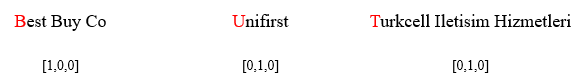
\includegraphics[scale=0.6]{figures/alphabet_order.png}
    \caption{Examples of alphabetical ordering}
    \label{fig:alphabeticalorder}
\end{figure}
\vspace{0.5cm}

\noindent

With this feature, we have to take into account which first letter we take. Stock overviews are usually sorted either based on names or based on ticker symbols. The first letter of the name may differ from that of the ticker, thereby resulting in different orderings. We choose to work with names since generally, name and ticker orderings are roughly the same. The latter can be checked by calculating Spearman's rho between the orderings obtained by sorting based on company names and tickers. The rho turns out to be 0.902 in our list of company names. The high correlation indicates that the orderings are roughly the same.


\subsubsection{Vowels and Consonants}
In almost every language, there is a distinction between vowels and consonants. This is the reason for introducing the vowel-to-length ratio. With this feature, we measure the vowel density of a word. The feature indirectly represents the consonant density as well, as the vowel density is linearly related to it. Examples of this feature are given in Figure \ref{fig:voweltolength} in which the vowels are marked in red.

\vspace{0.5cm}
\begin{figure}[h]
    \centering
    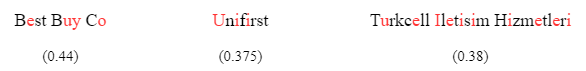
\includegraphics[scale=0.6]{figures/vowel_density.png}
    \caption{Examples of the vowel-to-length ratio}
    \label{fig:voweltolength}
\end{figure}
\vspace{0.5cm}




\newpage
\subsubsection{Repetition and Rhyme}
\cite{mcglone2000birds} have done an experiment from which they draw a relationship between rhyme and processing fluency. In the experiment, they let people rate the accuracy of pairs of aphorisms. One of them was rhyming, while the other did not. The meaning of the statements was kept the same. They find that people rate a rhyming statement as more true than its non-rhyming variant. In their study, they conclude that rhyme enhances processing fluency. As a proxy for such a rhyme factor, we chose to use the number of the most common letter in a firm name as a feature. This feature (in combination with other features) may capture the rhyme in a word. Figure \ref{fig:repetitions} gives some examples of this feature, where the most common letter is marked in red. Some words and names may have multiple most common letters.

\vspace{0.5cm}
\begin{figure}[h]
    \centering
    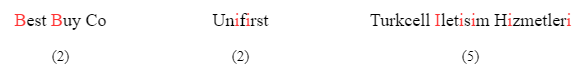
\includegraphics[scale=0.6]{figures/repetition.png}
    \caption{Examples of repetition and rhyme}
    \label{fig:repetitions}
\end{figure}
%\vspace{0.5cm}


\subsubsection{Spell-Check}
The last feature is the spell-check feature, which is inspired by the \textit{dictionary feature} of \cite{green2013company}. The principles are the same: if a set of words contains a word that the spell-checker marks as misspelled, then this feature takes the value 1. If no errors are detected, a value of 0 will be assigned. So, it is a binary variable that indicates whether a firm name contains spelling errors. One may interpret these spelling errors as a form of disfluency. The initial dictionary score is calculated with the Microsoft spell-checker and it is used as part of an unsupervised approach. In this paper, we use the \textit{Enchant} spell-checking library\footnote{\url{https://pypi.org/project/pyenchant/}}. The checks will be based on both an American English and British English dictionary. This means that if a word is correctly spelled in at least one of the two dictionaries, it will not be labelled as misspelled. Figure \ref{fig:haserrors} gives some examples of this feature. In red are the words that are marked as misspelled in English.

\vspace{0.5cm}
\begin{figure}[h]
    \centering
    
\includegraphics[scale=0.6]{figures/has_errors.png}
    \caption{Examples of spell-checking}
    \label{fig:haserrors}
\end{figure}
\vspace{0.5cm}



\newpage
\subsection{Deep Learning Model}

% https://keras.io/guides/keras_tuner/getting_started/#introduction
% https://keras.io/keras_tuner/
% https://machinelearningmastery.com/grid-search-hyperparameters-deep-learning-models-python-keras/

We now turn to the deep learning model, which we train with the frequency list (see \hyperref[Training set]{Section 3.2}). To do that, we first calculate the above-mentioned features for each word in the frequency list and standardise them. Then, we let the model fit those features on the frequencies of the words. In other words, we learn the model to determine a word's fluency (frequency) based on its standardised features. Once the model is trained, we use it to predict the fluency scores of company names. Important is the fact that we are assuming that the model, which is trained on words, is generalizable to (company) names. Since we are working at character and $n$-gram levels, we assume that the model is generalizable. The latter is because both the English words and names we use are constructed with the same elements from the same distribution (i.e., the letters from the English alphabet). Since this distribution is the same, one can argue that the strings constructed with it will also share the same properties. For instance, both words and names that contain less common $n$-grams will both be considered less English and/or fluent.

Implementing this deep learning model involves optimising a loss function. One of the most commonly used loss functions for training a regression neural network is the Mean Squared Error (MSE)
\begin{equation}
    MSE = \frac{1}{N}\sum_{i=1}^N(y_i - \hat{y}_i)^2
\end{equation}
in which $N$ is the total number of words/names, $y_i$ is the actual fluency score of observation $i$, and $\hat{y}_i$ is its predicted score. A disadvantage of using the MSE is that it is, due to its squaring, sensitive to outliers. Since we use frequency as the proxy for fluency, we notice that the distribution of word occurrences has similarities with a power law. This is no coincidence, as such power-like distributions are common among many empirical ranking datasets. A famous theory about this phenomenon is \textit{Zipf's law} \citep{zipf1932selected}, which states that frequency is inversely proportional to rank in a frequency list. This power behaviour of the data, together with the MSE, may cause the model to be biased toward the words that spike at the beginning of the list. To mitigate this issue, we use the more robust Mean Absolute Error (MAE) as loss and evaluation function instead
\begin{equation}
    MAE = \frac{1}{N}\sum_{i=1}^N|y_i - \hat{y}_i|
\end{equation}

In addition, we also need to tune the network's hyperparameters. To do that, we split the shuffled frequency list into 3 parts. 80\% is used to train the model during the hypertuning, 10\% is used as validation set during the hypertuning, and the last 10\% is used as test set to test the tuned model. In the hypertuning, we use 1000 random searches to search for the combination of hyperparameters that makes a model with the lowest validation loss.
We use 30 epochs to train the model and mini-batches of 100 observations.
We let the number of hidden layers vary over \{1,2,3,4,5\}. In each hidden layer, we choose between the ReLU activation function \citep{fukushima1975cognitron} and its smooth approximation, the Softplus activation function \citep{glorot2011deep}. The output layer has a linear activation function.
We search over \{4,8,16,32\} to find the optimal number of nodes per hidden layer, and we use $L1$-regularisation to address overfitting in each node. Both the learning rate of the Adam optimiser \citep{kingma2014adam} and the regularization parameter of the $L1$-regularisations are optimised over \{0.1, 0.01, 0.001\}. The implementation of the described framework is written in python\footnote{\url{https://github.com/KvnGitHubbb/ProFluency-Network.git}} and with use of Keras\footnote{\url{https://keras.io/}}$^,$\footnote{\url{https://github.com/keras-team/keras-tuner}}. The tuned network can be found in \hyperref[Appendix B]{Appendix B}.

Once the model is tuned and trained with 90\% of observations of the frequency list, we use the remaining 10\% to evaluate its out-of-sample performance. To do that, we use 4 benchmarks. The first benchmark is a uniform distribution that ranges from the minimum to the maximum fluency (frequency) scores that are present in the training observations. Based on that range, we assign random fluency scores to the test observations. The second benchmark is a normal distribution whose mean and standard deviation are the same as those of the fluency scores in the training set. Based on this normal distribution, we assign random fluency scores to the test observations.
The third benchmark samples with replacement from the fluency labels of the training observations. Each bootstrapped value is then randomly used as a fluency estimate for a test observation. The last benchmark is an Ordinary Least Squares (OLS) regression that is fitted on the training data. 

After this \textbf{intrinsic} evaluation, we re-estimate the weights of the tuned model using all the observations available in the frequency list. We use this model to predict company name fluency scores. 













\subsection{Evaluation of Fluency Score}
As we do not have ground truth fluency labels for the company names, we evaluate the company name fluency predictions \textbf{extrinsically} by examining how well these fluency scores explain stock characteristics. This is done with panel regressions. We regress monthly observations of stock characteristics on fluency scores and lagged control variables. 
The stock characteristics on which we focus are: valuation, liquidity, and performance.

\subsubsection{Valuation}
The market-to-book ratio shows how the market values a firm. The book value of a company is its value according to the balance sheet. It is calculated as total assets minus total liabilities. It can be interpreted as the company's net worth if it were to be completely liquidated. The market value indicates how much investors are willing to pay for a company. It is calculated as the stock price times the number of shares outstanding. This value may differ from the book value, as investors are usually forward-looking. The market-to-book ratio is obtained by dividing the market value by the book value. It can be interpreted as how much investors are willing to pay for each dollar in net assets.

A low market-to-book ratio could be a sign of undervaluation, while a high market-to-book value may indicate overvaluation. Since the valuation of a company is often very informative for investors, it is therefore worthwhile to investigate which factors influence it. 
The panel regression we use to examine the possible effect of firm name fluency on valuation is as follows:
\begin{equation}
    MB_{i,t} = \beta_1F_{i} + \boldsymbol{\beta_2'C_{i,t-1}} + \textit{Year Dummies} + \epsilon_{i,t}
\end{equation}
in which $MB_{i,t}$ is the market-to-book ratio of company $i$ in month $t$. $F_{i}$ is the predicted fluency score of company $i$. $\boldsymbol{C_{i,t-1}}$ is a vector containing control variables of company $i$ in month $t-1$. The \textit{Year Dummies} is a collection of 10 dummy variables that keep track of the years from 2013 to 2022. They serve as annual intercepts. We control each stock's valuation with the following variables:

\vspace{0.25cm}
\begin{itemize}
\setlength\itemsep{-0.5em}
    \item \begin{minipage}[t]{0.25\textwidth}
            Sales
        \end{minipage}
        \begin{minipage}[t]{0.5\textwidth}
            (\textit{sales/market capitalisation});
        \end{minipage}
        
    \item \begin{minipage}[t]{0.25\textwidth}
            Profitability
        \end{minipage}
        \begin{minipage}[t]{0.45\textwidth}
            (\textit{gross profit/total assets});
        \end{minipage}

    \item \begin{minipage}[t]{0.25\textwidth}
            Leverage
        \end{minipage}
        \begin{minipage}[t]{0.45\textwidth}
            (\textit{total debt/total assets}).
        \end{minipage}
\end{itemize}
\noindent
These control variables are also used in the study of \cite{green2013company} on the effect of firm name fluency on firm valuation. They originate from a collection of controls in the study by \cite{edmans2012real} which investigates the effects of valuation discounts on takeovers.






\subsubsection{Liquidity}
Another important stock characteristic is liquidity.
Liquidity is the ease with which assets can be bought or sold without large price changes. Investors should also take this characteristic into account, as illiquid assets could be more volatile or have higher transaction costs. To measure liquidity, we use the Amihud Illiquidity Measure \citep{amihud2002illiquidity}. This measure is one of the most commonly used illiquidity metrics in finance and it is calculated as the average ratio of absolute return to traded volume. In the original approach, this measure is calculated at annual intervals. Since we work with monthly observations, we transform the measure accordingly:

\begin{equation}
    ILLIQ_{i,t} = \frac{1}{D_t}\sum^{D_t}_{d=1} \frac{|r_{i,t,d}|}{V_{i,t,d}}
\end{equation}
The $ILLIQ_{i,t}$ is the illiquidity measure of stock $i$ in month $t$. $D_t$ is the number of trading days in month $t$ and $d$ is the index over those trading days. $r_{i,t,d}$ and $V_{i,t,d}$ is the gross return and traded volume of stock $i$ in month $t$ at day $d$, respectively. A stock with a relatively high illiquidity measure can be interpreted as relatively illiquid. This is because returns are relatively large in magnitude (large price changes) while volume is relatively low (little trading). An opposite interpretation holds when the illiquidity measure is low.

Like valuation, we use the same panel regression approach to examine the effect of company name fluency on liquidity: 
\begin{equation}
    \text{log}(\frac{1}{ILLIQ_{i,t}}) = \beta_1F_{i} + \boldsymbol{\beta_2'C_{i,t-1}} + \textit{Year Dummies} + \epsilon_{i,t}
\end{equation}
We use the log inverse illiquidity measure as dependent variable in (10) because this makes the regression more interpretable. The left-hand side in (10) can now be interpreted as a liquidity measure. Like valuation, We explain this measure using firm name fluency, yearly dummies and control variables. In this case, we control with:
\vspace{0.25cm}
\begin{itemize}
\setlength\itemsep{-0.5em}
    \item \begin{minipage}[t]{0.3\textwidth}
            Size
        \end{minipage}
        \begin{minipage}[t]{0.45\textwidth}
            (\text{log}(\textit{market capitalisation}));
        \end{minipage}
        
    \item \begin{minipage}[t]{0.3\textwidth}
            Profitability
        \end{minipage}
        \begin{minipage}[t]{0.45\textwidth}
            (\textit{gross profit/total assets});
        \end{minipage}
        
    \item \begin{minipage}[t]{0.3\textwidth}
            Valuation
        \end{minipage}
        \begin{minipage}[t]{0.45\textwidth}
           (\textit{market value/book value})
        \end{minipage}


    \item \begin{minipage}[t]{0.3\textwidth}
            Advertising
        \end{minipage}
        \begin{minipage}[t]{0.45\textwidth}
           (\textit{advertising expenses/sales});
        \end{minipage}

    \item \begin{minipage}[t]{0.3\textwidth}
            Price
        \end{minipage}
        \begin{minipage}[t]{0.45\textwidth}
           (\textit{1/market price});
        \end{minipage}
        
    \item \begin{minipage}[t]{0.3\textwidth}
            Volatility
        \end{minipage}
        \begin{minipage}[t]{0.45\textwidth}
            (\textit{monthly volatility}).
        \end{minipage}
\end{itemize}
\noindent
These control variables originate from the study by \cite{green2013company} in which they are used to evaluate the effect of firm name fluency on the number of retail and institutional shareholders. The researchers also have used these controls in their evaluation of the effects of fluency on trading (liquidity). The reason for this is that they assume that there are similarities in the way people make decisions about holding and trading stocks.




\subsubsection{Performance}
We also examine the potential effect of company name fluency on stock performance. With performance, we mean the realised monthly gross returns. Here, we also use a panel regression
\begin{equation}
    R_{i,t} = \beta_1F_{i} + \textit{Year Dummies} + \epsilon_{i,t}
\end{equation}
in which $R_{i,t}$ denotes the gross return of the stock of company $i$ in month $t$. Unlike the valuation and liquidity regressions, we do not include control variables in this regression. We assume that the annual dummies are sufficient in this setting, as returns are in general difficult to predict.




\newpage
\section{Results}
In this section, we first give the performance of the deep learning model for predicting the labels of the test set. Table \ref{tab:intrinsic} gives an overview of the out-of-sample performance compared to the benchmarks. Then, we provide the results of the panel regressions. More details about the fluency score predictions used in those regressions can be found in \hyperref[Appendix C]{Appendix C}.

\vspace{0.5cm}
\begin{table}[h]
\centering
\caption{Out-of-sample performance comparison}
\label{tab:intrinsic}
\begin{tabular}{lllllllllll}
\hline
    &  & \textbf{uniform}                     &                      & \textbf{normal}                    &                      & \textbf{bootstrap}                 &  & \textbf{OLS}   &                      & \textbf{deep learning}            \\ \hline
    &  &                             &                      &                           &                      &                           &  &       &                      &                          \\
MAE &  & \multicolumn{1}{c}{4408402} & \multicolumn{1}{c}{} & \multicolumn{1}{c}{88509} & \multicolumn{1}{c}{} & \multicolumn{1}{c}{10600} &  & 11183 & \multicolumn{1}{c}{} & \multicolumn{1}{c}{4951} \\
    &  &                             &                      &                           &                      &                           &  &       &                      &                          \\ \hline
\end{tabular}
\end{table}
\vspace{0.5cm}

Table \ref{tab:intrinsic} shows that the out-of-sample performance (measured by the MAE) improves as the model incorporates more information from the training set. The uniform model has by far the highest MAE, as this model only takes the range of fluency (frequency) scores into account. The normal model provides an improvement over the uniform model, as it gives less weight to the extreme values. It also works with the information that is contained in its mean and standard deviation. The bootstrap model in turn improves the normal model, as it also takes into account the shape of the fluency distribution. The performance of the OLS model comes close to that of the bootstrap model. The deep learning model has the best out-of-sample performance. Its MAE is about a thousand times smaller compared to that of the most naive model and about 2 times smaller compared to the most competitive benchmarks.  

From this point onwards, we will continue with the extrinsic evaluation (i.e., the panel regressions). 
Noticeable there, is the occurrence of correlated error terms. The latter can occur in two ways. The first form is that the residuals of the different firms are contemporaneously correlated (i.e., within month $t$). The second form is that the company's residuals are correlated with each other (i.e., within firm $i$). The first form seems to be controlled for by the regression, as its
severity and impact are not noticeably high. So, based on that, we assume that the residuals are in general independent \textbf{between} firms. However, the latter seems not to hold for the \textbf{within}-firm residuals. This is because observations (and therefore the prediction errors) of the same company are more likely to be similar. The fact that these within-firm residuals are correlated with each other has no impact on the estimated coefficients in (8), (10), and (11). Yet, it does affect their significance as it affects the covariance matrix estimate. To ensure that we get covariance matrix estimates that are robust to potential within-firm autocorrelation, we estimate it as in \cite{arellano1987computing}, which is based on 3 assumptions. The first assumption is error independence between firms. The second assumption allows autocorrelation and heteroscedasticity of arbitrary form for within-firm residuals. The third assumption states that the number of firms ($N$) is large. As we satisfy these assumptions, we decide to apply this covariance matrix approach. The panel regression results thereof are reported in Table \ref{tab: panelregression}.\\


\begin{table}[h]
\centering
    
\caption{Coefficient estimates of the panel regression of each characteristic}
\label{tab: panelregression}
\begin{tabular}{llclllc}
\toprule
                                          &  &                              &  & \multicolumn{1}{c}{\textbf{Characteristic}} &  &                              \\\cline{3-7}\\
                                          &  & Valuation                   &  & \multicolumn{1}{c}{Liquidity}               &  & Performance                  \\ \midrule
                                          % &  &                              &  & \multicolumn{1}{c}{}                        &  &                              \\ \midrule
\textbf{Coefficients}                     &  &                              &  & \multicolumn{1}{c}{}                        &  &                              \\ \midrule
\multicolumn{1}{l|}{}                     &  & \multicolumn{1}{l}{}         &  &                                             &  &                              \\
\multicolumn{1}{l|}{Fluency}              &  & \multicolumn{1}{l}{3.077e-4*} &  & 7.371e-5                                     &  & \multicolumn{1}{l}{-2.454e-5} \\
\multicolumn{1}{l|}{}                     &  & \multicolumn{1}{l}{}         &  &                                             &  &                              \\
\multicolumn{1}{l|}{Sales}                &  & \multicolumn{1}{l}{-0.388}   &  &                                             &  &                              \\
\multicolumn{1}{l|}{}                     &  & \multicolumn{1}{l}{}         &  &                                             &  &                              \\
\multicolumn{1}{l|}{Profitability}        &  & \multicolumn{1}{l}{5.521***} &  & -0.020                                      &  &                              \\
\multicolumn{1}{l|}{}                     &  & \multicolumn{1}{l}{}         &  &                                             &  &                              \\
\multicolumn{1}{l|}{Leverage}             &  & \multicolumn{1}{l}{6.079***} &  &                                             &  &                              \\
\multicolumn{1}{l|}{}                     &  &                              &  &                                             &  &                              \\
\multicolumn{1}{l|}{Advertising}          &  &                              &  & 0.865                                       &  &                              \\
\multicolumn{1}{l|}{}                     &  &                              &  &                                             &  &                              \\
\multicolumn{1}{l|}{Size}                 &  &                              &  & 0.936***                                    &  &                              \\
\multicolumn{1}{l|}{}                     &  &                              &  &                                             &  &                              \\
\multicolumn{1}{l|}{Valuation}            &  &                              &  & -0.034*                                     &  &                              \\
\multicolumn{1}{l|}{}                     &  &                              &  &                                             &  &                              \\
\multicolumn{1}{l|}{Price}                &  &                              &  & 5.947***                                    &  &                              \\
\multicolumn{1}{l|}{}                     &  &                              &  &                                             &  &                              \\
\multicolumn{1}{l|}{Volatility}           &  &                              &  & 0.109***                                    &  &                              \\
\multicolumn{1}{l|}{}                     &  &                              &  & \multicolumn{1}{c}{}                        &  &                              \\ \midrule
\textbf{Statistics}                       &  &                              &  & \multicolumn{1}{c}{}                        &  &                              \\ \midrule
\multicolumn{1}{l|}{}                     &  & \multicolumn{1}{l}{}         &  &                                             &  & \multicolumn{1}{l}{{\ul }}   \\
\multicolumn{1}{l|}{Number of observations}      &  & 167 $\times$ 119                    &  & \multicolumn{1}{c}{202 $\times$ 119}               &  & 951 $\times$ 119                    \\
\multicolumn{1}{l|}{$R^2$} &  & 0.123                        &  & \multicolumn{1}{c}{0.773}                   &  & 0.010                        \\
\multicolumn{1}{l|}{Durbin-Watson}       &  & 0.057                        &  & \multicolumn{1}{c}{0.178}                   &  & 2.123                        \\
\multicolumn{1}{l|}{}                     &  & \multicolumn{1}{l}{}         &  &                                             &  & \multicolumn{1}{l}{}         \\ \bottomrule
\end{tabular}

\vspace{0.25cm}
{%\raggedright 
\scriptsize \textit{Note.} results that are significant at 10\%, 5\% and 1\% significance level are displayed with a *, **, and ***, respectively. \par}
\end{table}\\

The headers under \textbf{Characteristic} indicate which stock characteristic is used as dependent variable in the regression. The rows under \textbf{Coefficients} give the estimated effects of the fluency scores and lagged control variables in each regression. We do not report the coefficients of the yearly dummy variables, as these can be interpreted as intercepts that deal with uncaptured (annual) common factors. For the reported estimates, we use asterisks to indicate their significance. Results that are significant at 10\%, 5\% and 1\% significance level are given with a *, **, and ***, respectively. The number of observations in each regression is equal to the number of companies times 119. That is because we lose one observation since we work with lagged explanatory variables (12 months $\times$ 10 years - 1 lag). In the following paragraphs, we evaluate the results of each regression.

In the valuation regression, we do find a (weak) significant effect of company name fluency on firm valuation ($p$ = 0.085). This implies that if a company's fluency score increases by 100, then its market value will increase by about 3.7\% of its book value.
This finding somewhat corresponds with the one in \cite{green2013company}. 
Aside from the differences in methods, They have found that an 1 unit increase in their fluency score results in a 2.53\% increase in the market-to-book ratio. When we look at the controls of this regression, we find that both profitability and leverage have significant effects on firm valuation.


In the liquidity regression we see that, in contrast to the finding in \cite{green2013company}, the fluency score has no significant effect on the liquidity measure. Liquidity is mainly explained by its (intuitive) control variables. First, companies with larger market capitalisation have more liquid stocks. Second, companies whose stock prices are relatively expensive are less liquid. Last, lagged volatility turns out to be positively correlated with current liquidity. 

In the performance column, we do again find results that are in line with both the return findings in \cite{green2013company} and more general ones in other literature. In fact, we conclude that returns are not predictable, at least not with the company name fluency scores predicted by our model. The latter can also be seen from the last $R^2$ under \textbf{Statistics}, which is, compared to the other two values, relatively low. The Durbin-Watson statistic of this regression has a value close to 2, which indicates that the residuals in the performance regression are not autocorrelated. The Durbin-Watson statistics of the other two regressions are an indication of positive (within-firm) autocorrelation. This also supports the use of the adjusted covariance matrix estimate. 






\newpage
\section{Conclusion}
In this paper, we have examined the effect of company name fluency on stock characteristics. The evaluated characteristics are valuation, liquidity, and performance.
First, we have made features based on insights from behavioural finance. Then, we use those features to train a deep learning model. We have done that with an English frequency list, in which the features of the words serve as input. The word frequencies are used as a proxy for the fluency target. We first evaluated the out-of-sample performance of this deep learning model intrinsically with the test set. Then, we use the trained model to predict name fluency scores of the companies that are listed on the New York Stock Exchange. We have examined the effects of those predictions extrinsically with panel regressions. In these regressions, we regress the company stock characteristics on the predicted fluency scores and control variables.

The results show that the deep learning model is able to beat the naive benchmarks regarding the out-of-sample performance. This means that the deep learning model is able to effectively use its layered structure to get better estimates of the fluency (frequency) scores of words compared to the random and/or naive benchmarks. 

In the panel regressions, we see that the model's fluency predictions only have significant effects in the case of valuation. In the case of liquidity, we find that company size, stock price, and volatility have strong significant regression coefficients instead. For performance, we also observe no significance of the fluency predictions, this is likely due to the fact that returns are very difficult to predict.

The main implication of this research is therefore that investors could get a rough insight into a company's valuation by looking at its name. Intuitively guessing the name fluency requires little to no skill, thus making it an easy and convenient evaluation tool. Besides that, one should also still focus on well-established and fundamental financial aspects, like profitability or size, when evaluating firms. 

In addition to fluency scores, the deep learning framework may also be relevant as we have shown that it is able to predict the fluency (frequency) of words reasonably well. Improved versions of this framework can become useful in other applications such as generative A.I. or text editors.

At last, there were also some limitations in this study. First, we have only considered companies that have been in existence for at least 10 years. This can cause an age bias, as previous research has shown that name effects are particularly strong during the first periods after the IPO. Furthermore, we have worked with a reduced amount of observations as we only used completely balanced panels. Finally, we also have only evaluated the fluency of words from an English perspective. Words and names that are not fluent in English may be more fluent in other languages.
Further research can be done in which such limitations are mitigated or resolved.



























%%%%%%%%%%%%%%%%%%%%%%%%%%%%%%%%%%%%%%%%%%%%%%%%%%%%%%%%%%%%%%%%%%%
\newpage
\bibliographystyle{abbrvnat}
\bibliography{library}




\newpage
\section*{Appendix A: Englishness Scores}\label{Appendix A}
To give an intuition of the Englishness score, we sort the firms based on their scores and present the top 10, the 10 companies around the median and the last 10 companies in Table \ref{tab: englishness scores}. Due to the negative log-likelihood, words with lower Englishness scores are considered more English.

\vspace{1cm}
\begin{center}
\begin{table}[h]
\caption{Examples of the Englishness score}
\label{tab: englishness scores}
\scalebox{0.9}{
\begin{tabular}{clccc}
\toprule
\textbf{top 10}                    &  & \textbf{median 10}          & \multicolumn{1}{l}{} & \textbf{last 10}               \\ \midrule
The Bank of New York Mellon        &  & Discover Financial Services &                      & DXC Technology Company         \\
(-23.407)                          &  & (-0.145)                    &                      & (17.536)                       \\
\multicolumn{1}{l}{}               &  &                             &                      &                                \\
ASA Gold and Precious Metals       &  & Renren                      &                      & LTC Properties                 \\
(-19.479)                          &  & (-0.142)                    &                      & (18.577)                       \\
\multicolumn{1}{l}{}               &  &                             &                      &                                \\
Fresh Del Monte Produce            &  & Yelp                        &                      & HCA Healthcare                 \\
(-17.657)                          &  & (-0.134)                    &                      & (19.006)                       \\
\multicolumn{1}{l}{}               &  &                             &                      &                                \\
The Procter Gamble Company         &  & Unifirst                    &                      & Mitsubishi UFJ Financial Group \\
(-16.943)                          &  & (-0.102)                    &                      & (19.334)                       \\
\multicolumn{1}{l}{}               &  &                             &                      &                                \\
The St Joe Company                 &  & Tegna                       &                      & PPG Industries                 \\
(-16.812)                          &  & (-0.080)                    &                      & (19.625)                       \\
\multicolumn{1}{l}{}               &  &                             &                      &                                \\
Canadian Imperial Bank of Commerce &  & DHI Group                   &                      & LSB Industries                 \\
(-16.568)                          &  & (-0.070)                    &                      & (19.755)                       \\
\multicolumn{1}{l}{}               &  &                             &                      &                                \\
The Coca Cola Company              &  & Carpenter Technology        &                      & LyondellBasell Industries       \\
(-16.489)                          &  & (-0.069)                    &                      & (19.816)                       \\
\multicolumn{1}{l}{}               &  & \multicolumn{1}{l}{}        & \multicolumn{1}{l}{} & \multicolumn{1}{l}{}           \\
Banco De Chile                     &  & Itau Unibanco Banco Holding &                      & PT Telekomunikasi Indonesia    \\
(-16.112)                          &  & (-0.057)                    &                      & (20.577)                       \\
\multicolumn{1}{l}{}               &  &                             &                      &                                \\
Best Buy Co                        &  & Banco Brasdesco             &                      & BWX Technologies               \\
(-15.762)                          &  & (-0.035)                    &                      & (23.886)                       \\
\multicolumn{1}{l}{}               &  &                             &                      &                                \\
Eli Lilly and Company              &  & Regal Rexnord               &                      & Turkcell Iletisim Hizmetleri   \\
(-15.688)                          &  & (-0.012)                    &                      & (27.183)                       \\ \bottomrule
\end{tabular}
}






\end{table}
\end{center}
















\newpage
\section*{Appendix B: Tuned Hyperparameters}\label{Appendix B}
An overview of the tuned hyperparameters is given in Table \ref{tab:hyperparameters}. In the \textbf{Structure} column, we indicate at which level in the network we have tuned the hyperparameters. The \textbf{Hyperparameter} column shows which hyperparameters are tuned. The tuned value of each hyperparameter is given in the last column. 


\vspace{1cm}
\begin{table}[h]
\begin{center}
\caption{Tuned hyperparameters of the deep learning model}
\label{tab:hyperparameters}
\begin{tabular}{llllcl}
\toprule
\multicolumn{1}{c}{\textbf{Structure}} & \multicolumn{1}{c}{} & \multicolumn{1}{c}{\textbf{Hyperparameter}} & \multicolumn{1}{c}{} & value                & \multicolumn{1}{c}{} \\ \midrule
                              &                      &                                    &                      & \multicolumn{1}{l}{} &                      \\
Layer 1                       &                      & Amount of nodes                    &                      & 16                   &                      \\
                              &                      & $L1$ regularisation                &                      & 0.001                &                      \\
                              &                      & Activation function                &                      & Softplus             &                      \\
                              &                      &                                    &                      &                      &                      \\
Layer 2                       &                      & Amount of nodes                    &                      & 32                   &                      \\
                              &                      & $L1$ regularisation                &                      & 0.01                 &                      \\
                              &                      & Activation function                &                      & ReLU                 &                      \\
                              &                      &                                    &                      &                      &                      \\
Layer 3                       &                      & Amount of nodes                    &                      & 16                   &                      \\
                              &                      & $L1$ regularisation                &                      & 0.01                 &                      \\
                              &                      & Activation function                &                      & ReLU                 &                      \\
                              &                      &                                    &                      &                      &                      \\
Layer 4                       &                      & Amount of nodes                    &                      & 8                    &                      \\
                              &                      & $L1$ regularisation                &                      & 0.001                &                      \\
                              &                      & Activation function                &                      & ReLU                 &                      \\
                              &                      &                                    &                      &                      &                      \\ \midrule
Network                       &                      & Amount of  hidden layers           &                      & 4                    &                      \\
                              &                      & Learning rate                      &                      & 0.1                  &                      \\ \bottomrule
\end{tabular}
\end{center}
\end{table}
\vspace{1cm}














\newpage
\section*{Appendix C: Predicted Fluency Scores}\label{Appendix C}
To give an insight into the predicted fluency scores, we plot its histogram in Figure \ref{fig:histogram}. The $x$-axis shows the fluency score buckets and the $y$-axis shows how many predictions each bucket has. Table \ref{tab:my-table summary stat} gives some summary statistics of the fluency score distribution. From both Figure \ref{fig:histogram} and Table \ref{tab:my-table summary stat} we see that the distribution is skewed to the left (i.e., to lower fluency scores).

\vspace{1cm}
\begin{figure}[h]
    \centering
    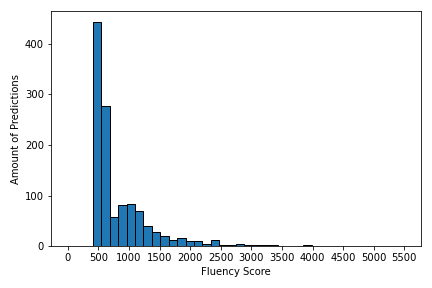
\includegraphics[scale=0.8]{figures/hist.png}
    \caption{Histogram of the fluency score predictions }
    \label{fig:histogram}
\end{figure}
\vspace{1cm}


\begin{table}[h]
\centering
\caption{Summary statistics of the fluency score predictions}
\label{tab:my-table summary stat}
\begin{tabular}{llc}
\toprule
\textbf{Statistic} &  &value \\ \midrule
          &  &           \\
Mean      &  & 826.558   \\
Median    &  & 622.616   \\
Min       &  & 424.110   \\
Max       &  & 5282.797  \\
Std. Dev. &  & 566.358   \\ 
\\ \bottomrule
\end{tabular}
\end{table}






\end{document}











